\documentclass[11pt]{article}
\usepackage[utf8]{inputenc}
\usepackage[russian]{babel}
\usepackage{float}
\usepackage{url}
\usepackage{amsmath}
\usepackage{amssymb}
\usepackage{graphicx}

\usepackage{setspace}
% полуторный интервал
\onehalfspacing


\usepackage{geometry}
 \geometry{
 a4paper,
 total={170mm,257mm},
 left=25mm,
 top=36mm,
 bottom=36mm,
 right=25mm
 }
\newcommand{\rom}[1]{\uppercase\expandafter{\romannumeral #1\relax}}

\renewenvironment{abstract}
    {\par\noindent\textbf{\abstractname.}\ \ignorespaces}
 
\newcommand{\keywords}[1]
    {\par\noindent\textbf{Ключевые слова:} #1}

\usepackage{fontspec}
\setmainfont{Times New Roman}

\title{Отчёт о исследовании тональности в кризисных твитах}
\author{
        Д. С. Ларионов$^{\rom{1}, \rom{2}}$, И. В. Смирнов$^{\rom{1}, \rom{2}}$\\
        $^{\rom{1}}$ Федеральное государственное учреждение \\"Федеральный Исследовательский Центр "Информатика и Управление"\\ Российской академии наук" \\
        $^{\rom{2}}$ Российский Университет Дружбы Народов
}
\date{\today}

\begin{document}
\maketitle
\newpage
\tableofcontents
\newpage

%\begin{abstract}
%This is the paper's abstract \ldots
%\end{abstract}

%\keywords{бла, бла-бла, бла-бла-бла}

\section{Введение}
\par В данном отчете в разделах 2-3 будут описаны данные и методы, использованные при проведении исследования о выявлении статистических значимых различий в тональности, полярности, субъективности и иных параметров текстов постов в социальной сети Твиттер\footnote{\url{https://twitter.com}}, так или иначе связанных с чрезвычайными ситуациями различного масштаба, характера и значимости.
\par Далее, в разделах 4-5 будут приведены результаты исследования в виде графиков и значений критериев стат. значимости.

\section{Данные}

Для данного исследования был выбран известный набор данных CrisisLexT6 \footnote{\url{https://crisislex.org/data-collections.html#CrisisLexT6}} \cite{olteanu2014crisislex}.  Набор состоит из 60000 твитов на английском языке, промаркированных по релевантности и сгруппированных по 6 чрезвычайным происшествиям, имевшим место в США, Канаде и Австралии в период с 2012 по 2013:
\begin{itemize}
    \item 2012 Ураган Сэнди - 6138 релевантных твитов (в результатах: sandy\_hurricane). Мощный тропический циклон. Подробнее: \url{https://en.wikipedia.org/wiki/Hurricane_Sandy}.
    \item 2013 Теракт во время Бостонского Марафона  - 5648 твитов  (boston\_bombings). \url{https://en.wikipedia.org/wiki/Boston_Marathon_bombing}.
    \item 2013 Торнадо в Оклахоме - 4827 твитов (oklahoma\_tornado). Массивный торнадо, ударивший по городу Мур в штате Оклахома. \url{https://en.wikipedia.org/wiki/2013_Moore_tornado}.
    \item 2013 Взрыв на Западном Техасе - 5246 твитов  (texas\_explosion). Взрыв нитрата аммония на заводе удобрений. \url{https://en.wikipedia.org/wiki/West_Fertilizer_Company_explosion}.
    \item 2013 Наводнения в Альберте - 5189 твитов (alberta\_floods). \url{https://en.wikipedia.org/wiki/2013_Alberta_floods}.
    \item 2013 Наводнения в Квинсленде - 5414 твитов (queensland\_floods). \url{https://en.wikipedia.org/wiki/Cyclone_Oswald}.
    
\end{itemize}

Для каждого проишествия из всех твитов, к нему относящихся, были выбраны только релевантные.

\section{Методы}
Использованные методы можно разделить на три категории:
\begin{enumerate}
    \item Статистический анализ по словарям с помощью LIWC.
    \item Статистический анализ с помощью словарей полярности и субъективности.
    \item Анализ с применением предобученной нейросетевой модели.
\end{enumerate}

\subsection{Статистический анализ по словарям с помощью LIWC}
Был использован пакет LIWC 2015\footnote{\url{http://liwc.wpengine.com/}}, версия 1.6, в варианте 30-дневной аренды для академических целей. Руководство по интерпретации значений из LIWC находится на сайте \footnote{\url{http://liwc.wpengine.com/interpreting-liwc-output/}}.

\subsection{Статистический анализ с помощью словарей полярности и субъективности.}
Данный вид анализа был использован для определений показателей полярности и субъективности текста, написанного пользователем. Для данных целей была применена библиотека TextBlob для языка python. Её модуль, реализующий анализ полярности и субъективно опирается на подсчет числа слов из соотв. словарей, встречающихся в анализируемом примере(подробнее см. \footnote{\url{https://www.clips.uantwerpen.be/pages/pattern-en#sentiment}}). На выходе получаются два значения: первое принимает значения на отрезке $[-1.0, 1.0]$ и определяет полярность текста, второе принимает значение на отрезке $[0.0, 1.0]$ и определяет субъективность текста, где 0 - очень объективный текст, а 1 - очень субъективный. Словари собраны путем анализа отзывов о продуктах.

\subsection{Анализ с применением предобученной нейросетевой модели.}
Также для анализа текстов была применена предобученная нейросетевая модель из фреймворка Flair\footnote{\url{https://github.com/zalandoresearch/flair}} \cite{akbik-etal-2019-flair} от ZalandoResearch. Модель состоит из энкодера, предобученного на задаче языкового моделирования на корпусе англоязычных новостей и классификатора, предобученного на датасете англоязычных отзывов к фильмам с сайта IMDB, промаркированных по полярности. Для каждого текста модель предсказывает два значения: полярность текста(sentiment\_value) (POSITIVE либо NEGATIVE) и показатель sentiment\_score, который может быть интерпретирован как уверенность модели в предсказанной полярности, равно как и показатель того, насколько анализируемый текст соответствует предсказанной полярности. Помимо двух вышеописанных показателей, для каждого текста была рассчитана их комбинация по следующей формуле:

$$
fine\_sentiment(text) = 
\begin{cases}
1 \cdot sentiment\_score(text), \text{если } sentiment\_value(text) = `POSITIVE` \\[6pt]
-1 \cdot sentiment\_score(text), \text{если } sentiment\_value(text) = `NEGATIVE`
\end{cases}
$$


\section{Результаты анализа}

\subsection{LIWC}
Ввиду того, что в твиттере используется крайне специфичный лексикон, методы, основанные на словарях, могут иногда давать неинформативные результаты. Это крайне зависит от качества составления словаря и использованных при этом источников. В случае LIWC значения большинства показателей варьируются около нуля. Мы не приводим графики распределений всех 93 параметров и значения критерия стат.значимости  ввиду их количества. Тем не менее они могут быть построены в любом табличном процессоре на основе предоставленных нами таблиц с результатами анализа.

В конце отчета приведены графики распределений для некоторых выбранных нами показателей: posemo, negemo, risk (см. Рис. \ref{posemo}, \ref{negemo}, \ref{risk}).


Для них же приведем результаты попарного сравнения по двустороннему критерию Манна-Уитни для определения статистической значимости отличий. Принят уровень стат. значимости $\alpha = 0.05$.
\begin{itemize}
    \item Показатель `posemo`: - Статистически не значимые отличия между:\\
    boston\_bombings и queensland\_flood (U-статистика: 15452467.5, p-value: 0.2085) \\
    oklahoma\_tornado и alberta\_floods (U-статистика: 12284022.0, p-value: 0.0664) \\
    Во всех остальных парах статистически значимые отличия.
    
    \item Показатель `negemo`: - Во всех парах событий статистически значимые отличия.
    
    \item Показатель `risk`: - Статистически не значимые отличия между:\\
    boston\_bombings и alberta\_floods (U-статистика: 14536916.0, p-value: 0.1682) \\
    oklahoma\_tornado и alberta\_floods (U-статистика: 12581712.5, p-value: 0.4535) \\
    Во всех остальных парах статистически значимые отличия.
\end{itemize}

\subsection{Полярность и Субъективность с помощью словарей}

К данному методу применимы те же замечания, что и к предыдущему: метод, основанный на работе с предварительно составленным лексиконом может не всегда давать информативные результаты применительно к текстам из социальных сетей.

Ниже приведены графики распределений показателей полярности и субъективности (см. Рис. \ref{polarity}, \ref{subjectivity}).

А так же результаты попарного сравнения по двустороннему критерию Манна-Уитни для определения статистической значимости отличий. Принят уровень стат. значимости $\alpha = 0.05$.

\begin{itemize}
    \item Показатель полярности: - Статистически не значимые отличия между:\\
    sandy\_hurricane и oklahoma\_tornado (U-статистика: 14679290.0, p-value: 0.3913) \\
    texas\_explosion и boston\_bombings (U-статистика: 14801308.0, p-value: 0.9321) \\
    Во всех остальных парах статистически значимые отличия.
    
    \item Показатель субъективности: - Статистически не значимые отличия между:\\
    sandy\_hurricane и alberta\_floods (U-статистика: 16253076.5, p-value: 0.0517) \\
    sandy\_hurricane и texas\_explosion (U-статистика: 15878924.0, p-value: 0.1948) \\
    oklahoma\_tornado и alberta\_floods (U-статистика: 12428549.0, p-value: 0.4964) \\
    oklahoma\_tornado и queensland\_flood (U-статистика: 13027372.5, p-value: 0.7850) \\
    alberta\_floods и queensland\_flood (U-статистика: 14098774.0, p-value: 0.7326) \\
    Во всех остальных парах статистически значимые отличия.
\end{itemize}

\subsection{Sentiment-анализ с помощью нейронных сетей}

Для демонстрации результатов данного подходы мы приведем графики (см. Рис. \ref{fine_sentiment}) и результаты сравнения только для показателя fine\_sentiment поскольку он является комбинацией двух других показателей.

Ниже приведены результаты попарного сравнения по двустороннему критерию Манна-Уитни для определения статистической значимости отличий. Принят уровень стат. значимости $\alpha = 0.05$.

Статистически не значимые отличия между:\\
    sandy\_hurricane и texas\_explosion (U-статистика: 16164525.0, p-value: 0.7118) \\
    oklahoma\_tornado и alberta\_floods (U-статистика: 12549107.0, p-value: 0.8602) \\
    oklahoma\_tornado и boston\_bombings (U-статистика: 13884129.0, p-value: 0.1014) \\
    alberta\_floods и boston\_bombings (U-статистика: 14885558.0, p-value: 0.1541) \\
    
    Во всех остальных парах статистически значимые отличия.



\bibliographystyle{abbrv}
\bibliography{main}

\begin{figure}
\centering
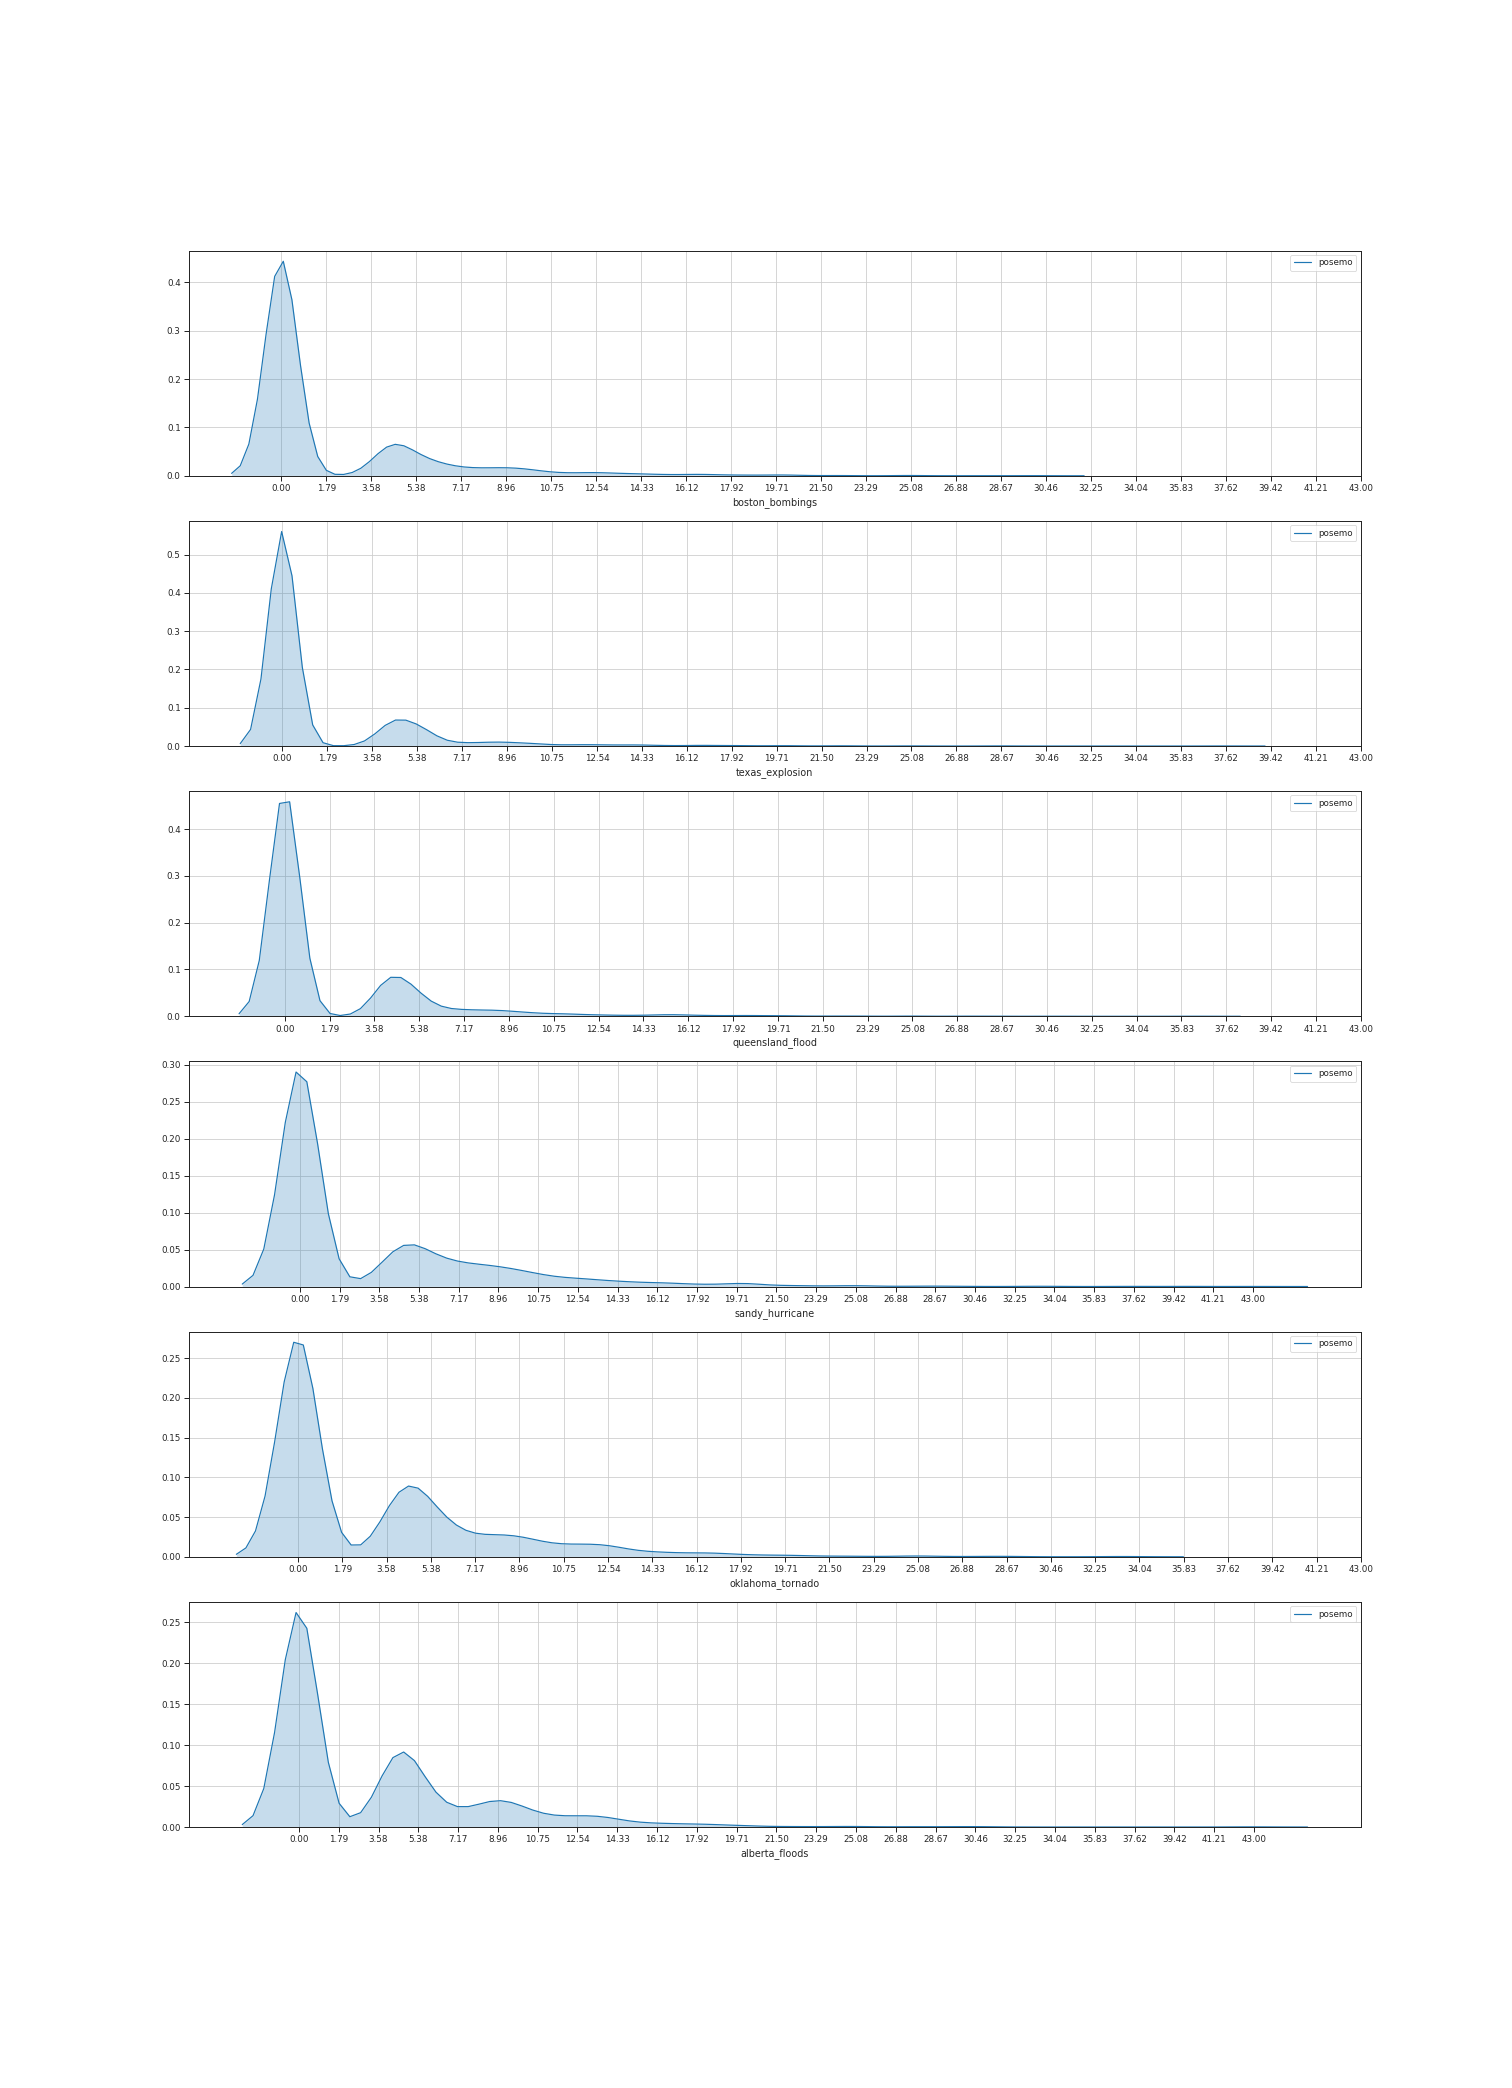
\includegraphics[width=\textwidth]{posemo.png}
\caption{Показатель `posemo` - позитивные эмоции}\label{posemo}
\end{figure}

\begin{figure}
\centering
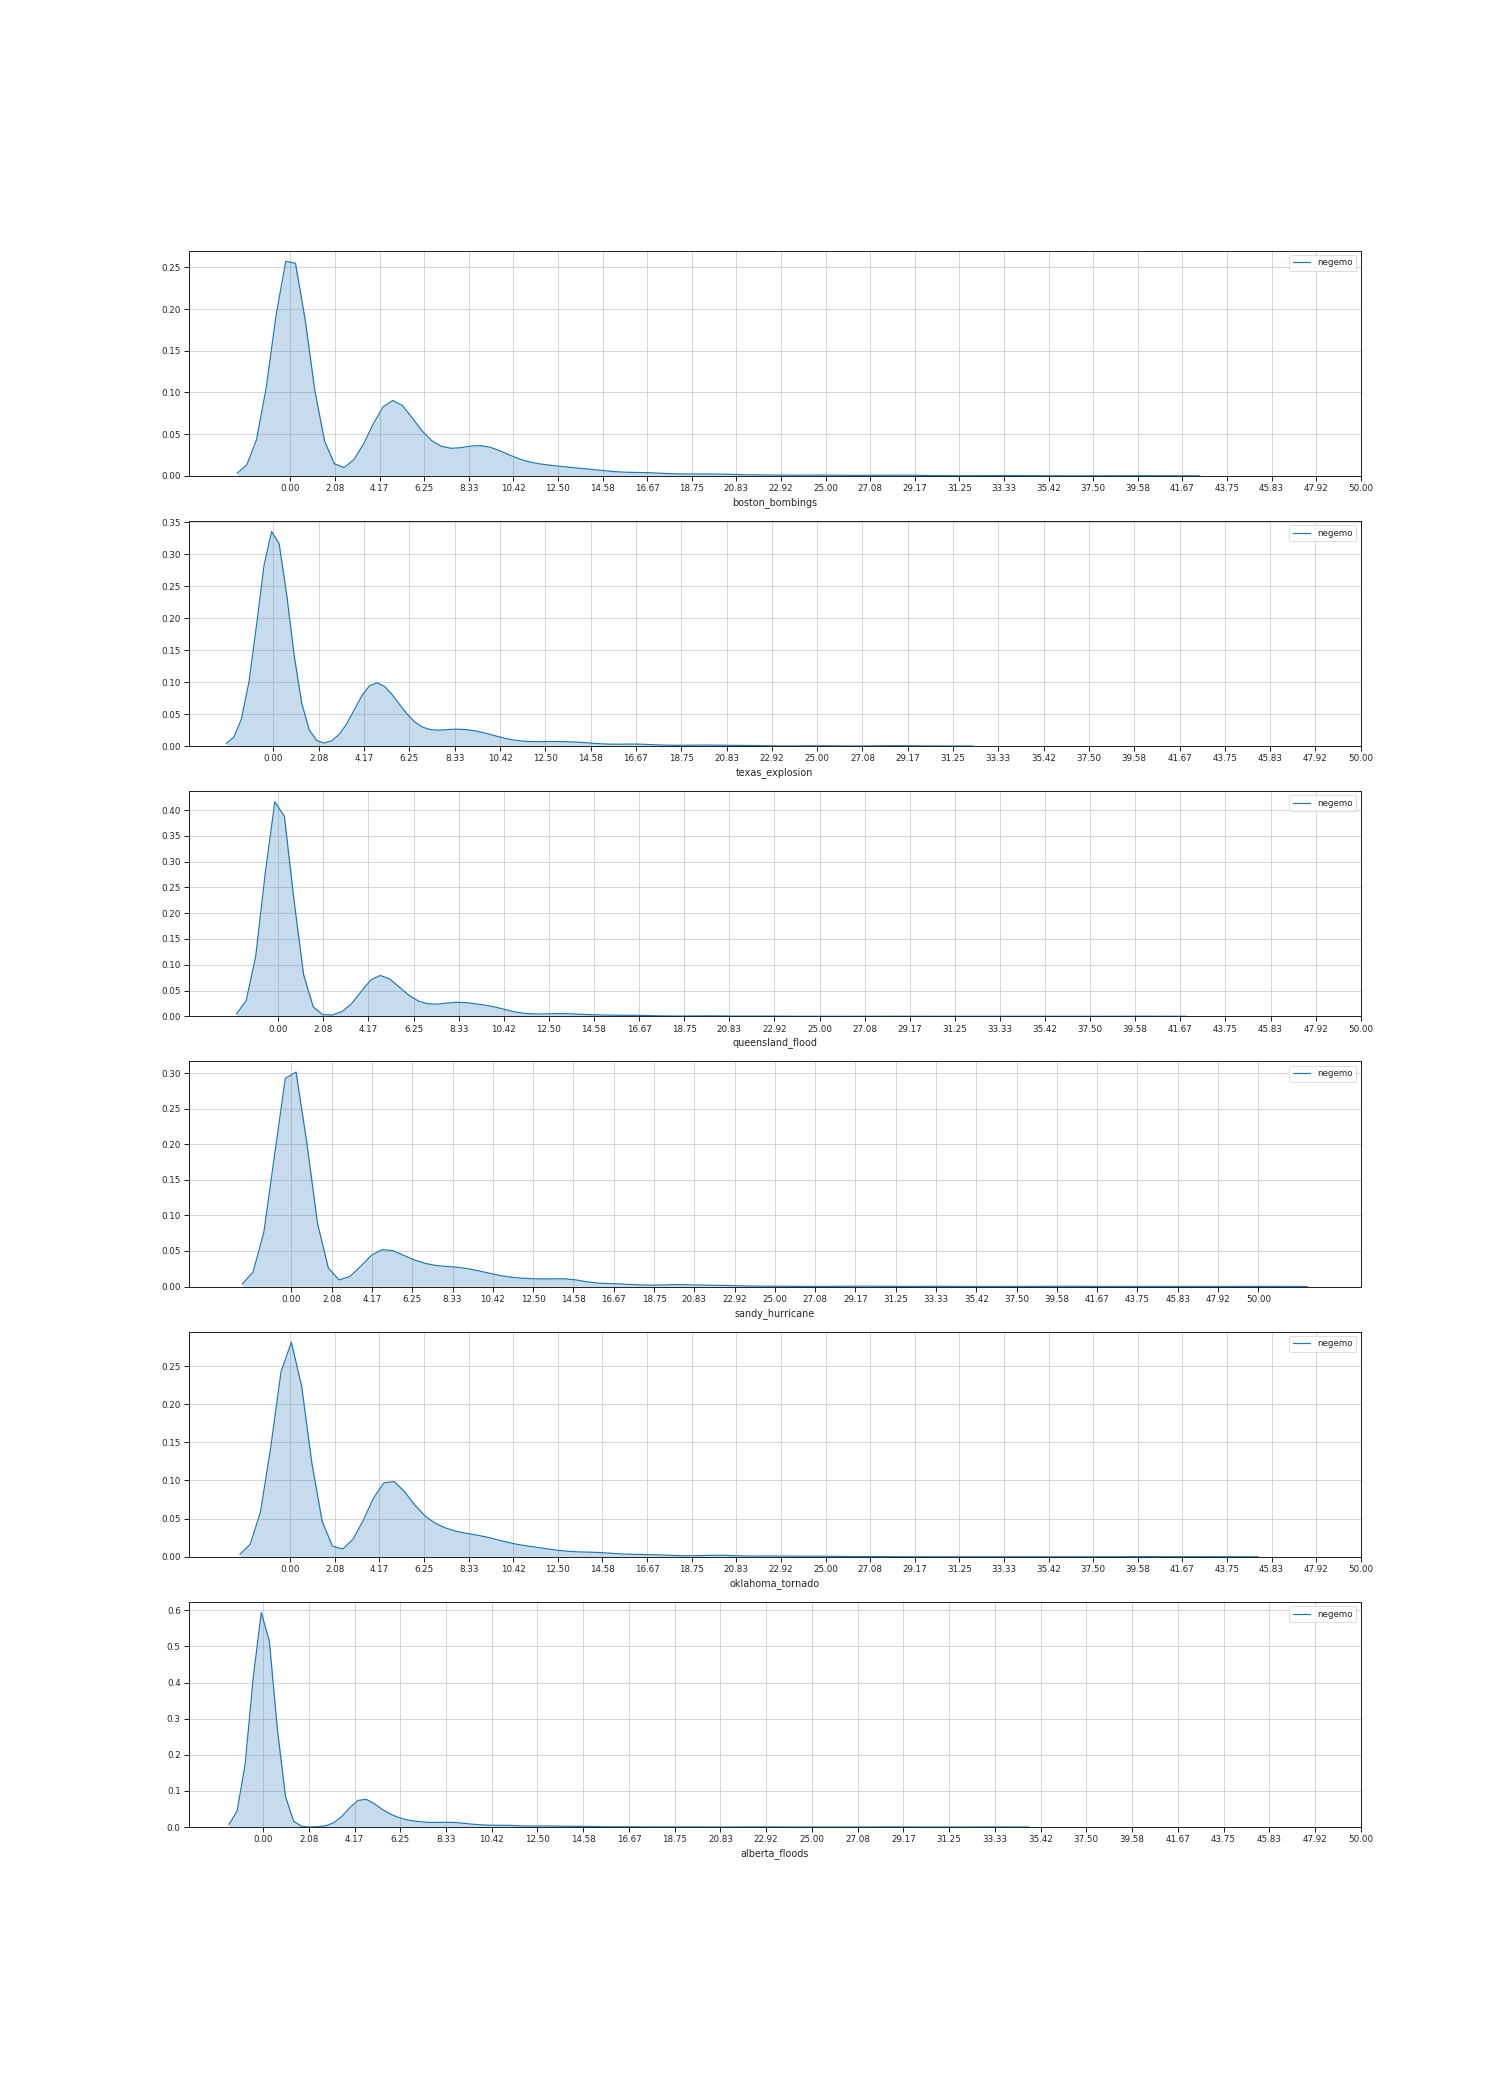
\includegraphics[width=\textwidth]{negemo.png}
\caption{Показатель `negemo` - негативные эмоции}\label{negemo}
\end{figure}

\begin{figure}
\centering
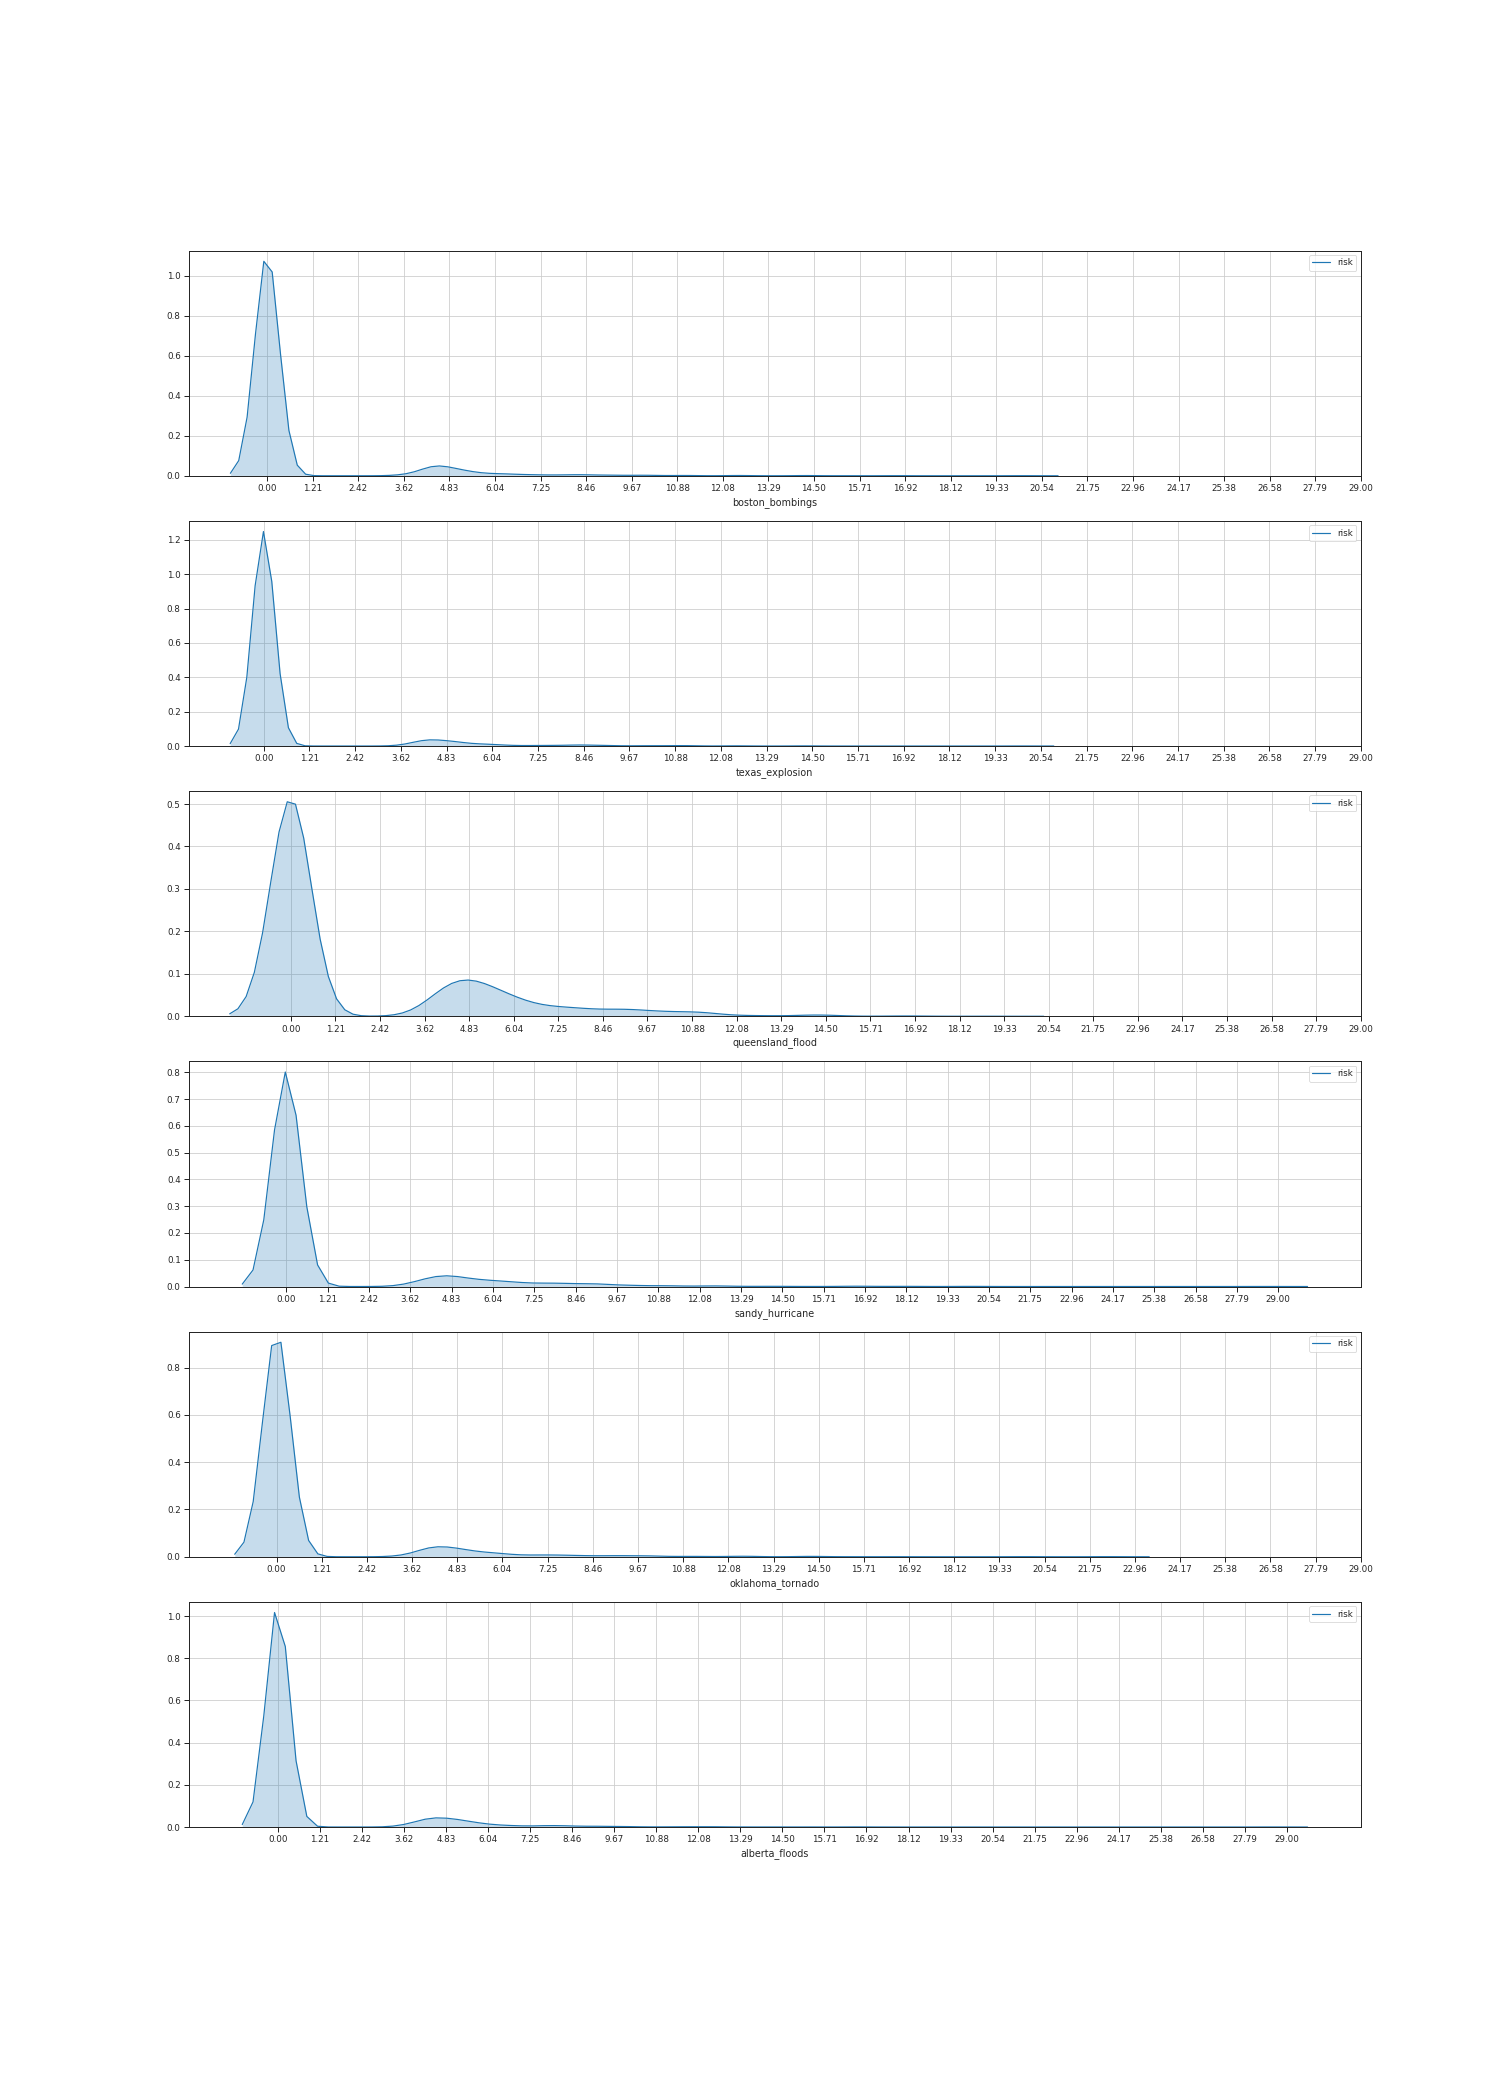
\includegraphics[width=\textwidth]{risk.png}
\caption{Показатель `risk`}\label{risk}
\end{figure}

\begin{figure}
\centering
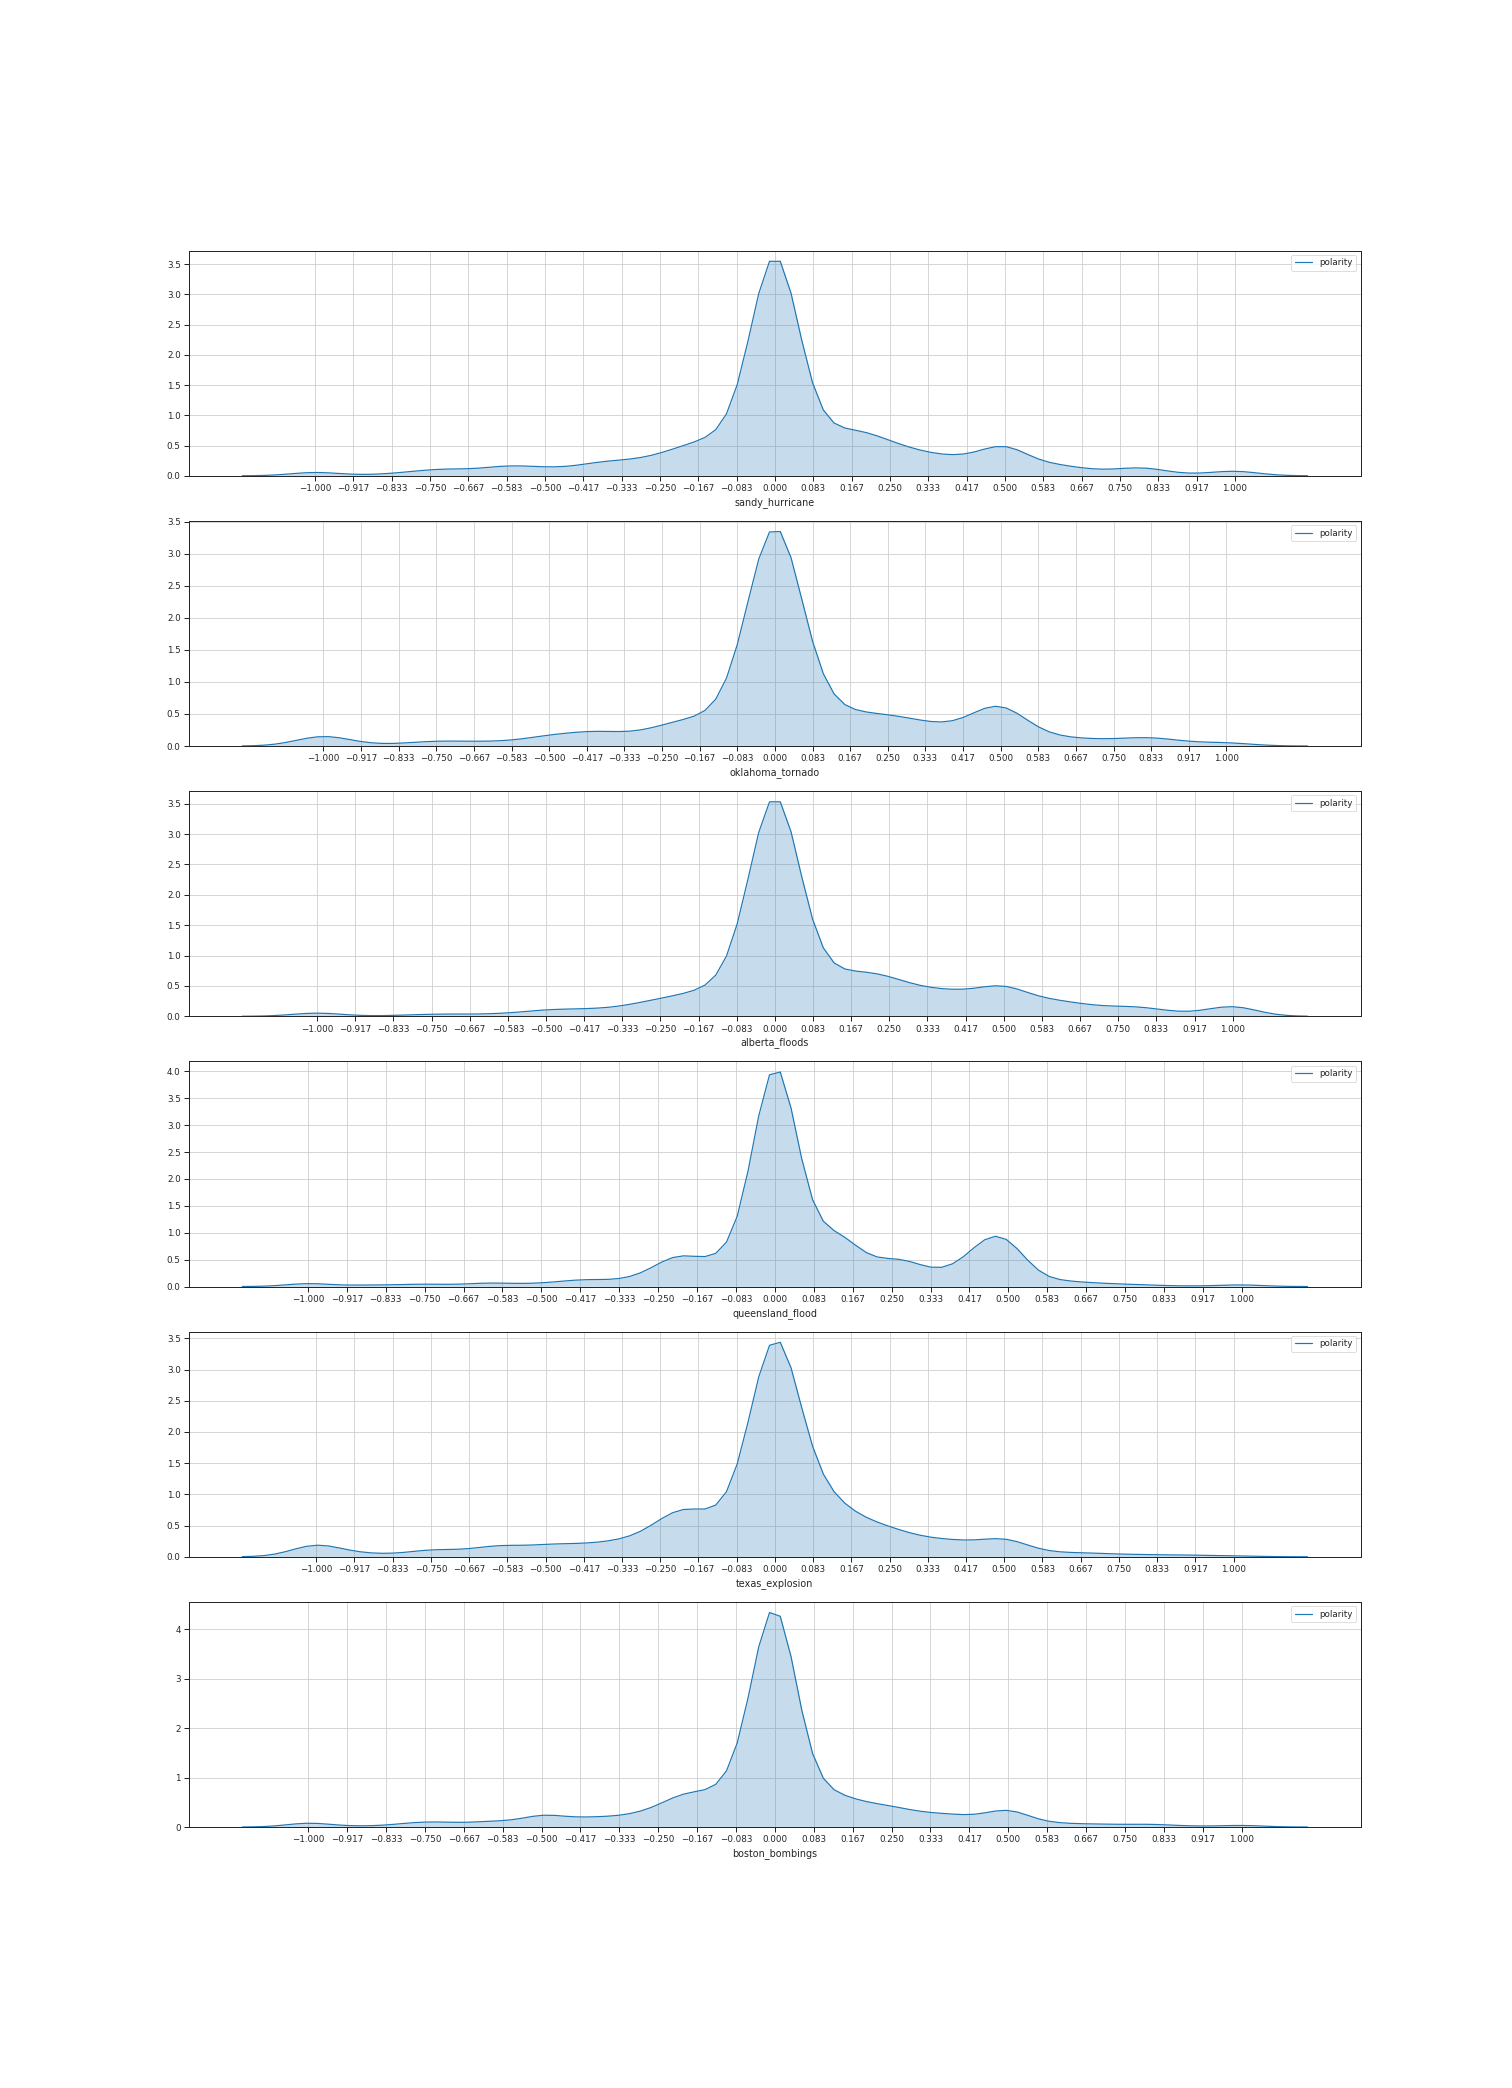
\includegraphics[width=\textwidth]{polarity.png}
\caption{Показатель полярности}\label{polarity}
\end{figure}

\begin{figure}
\centering
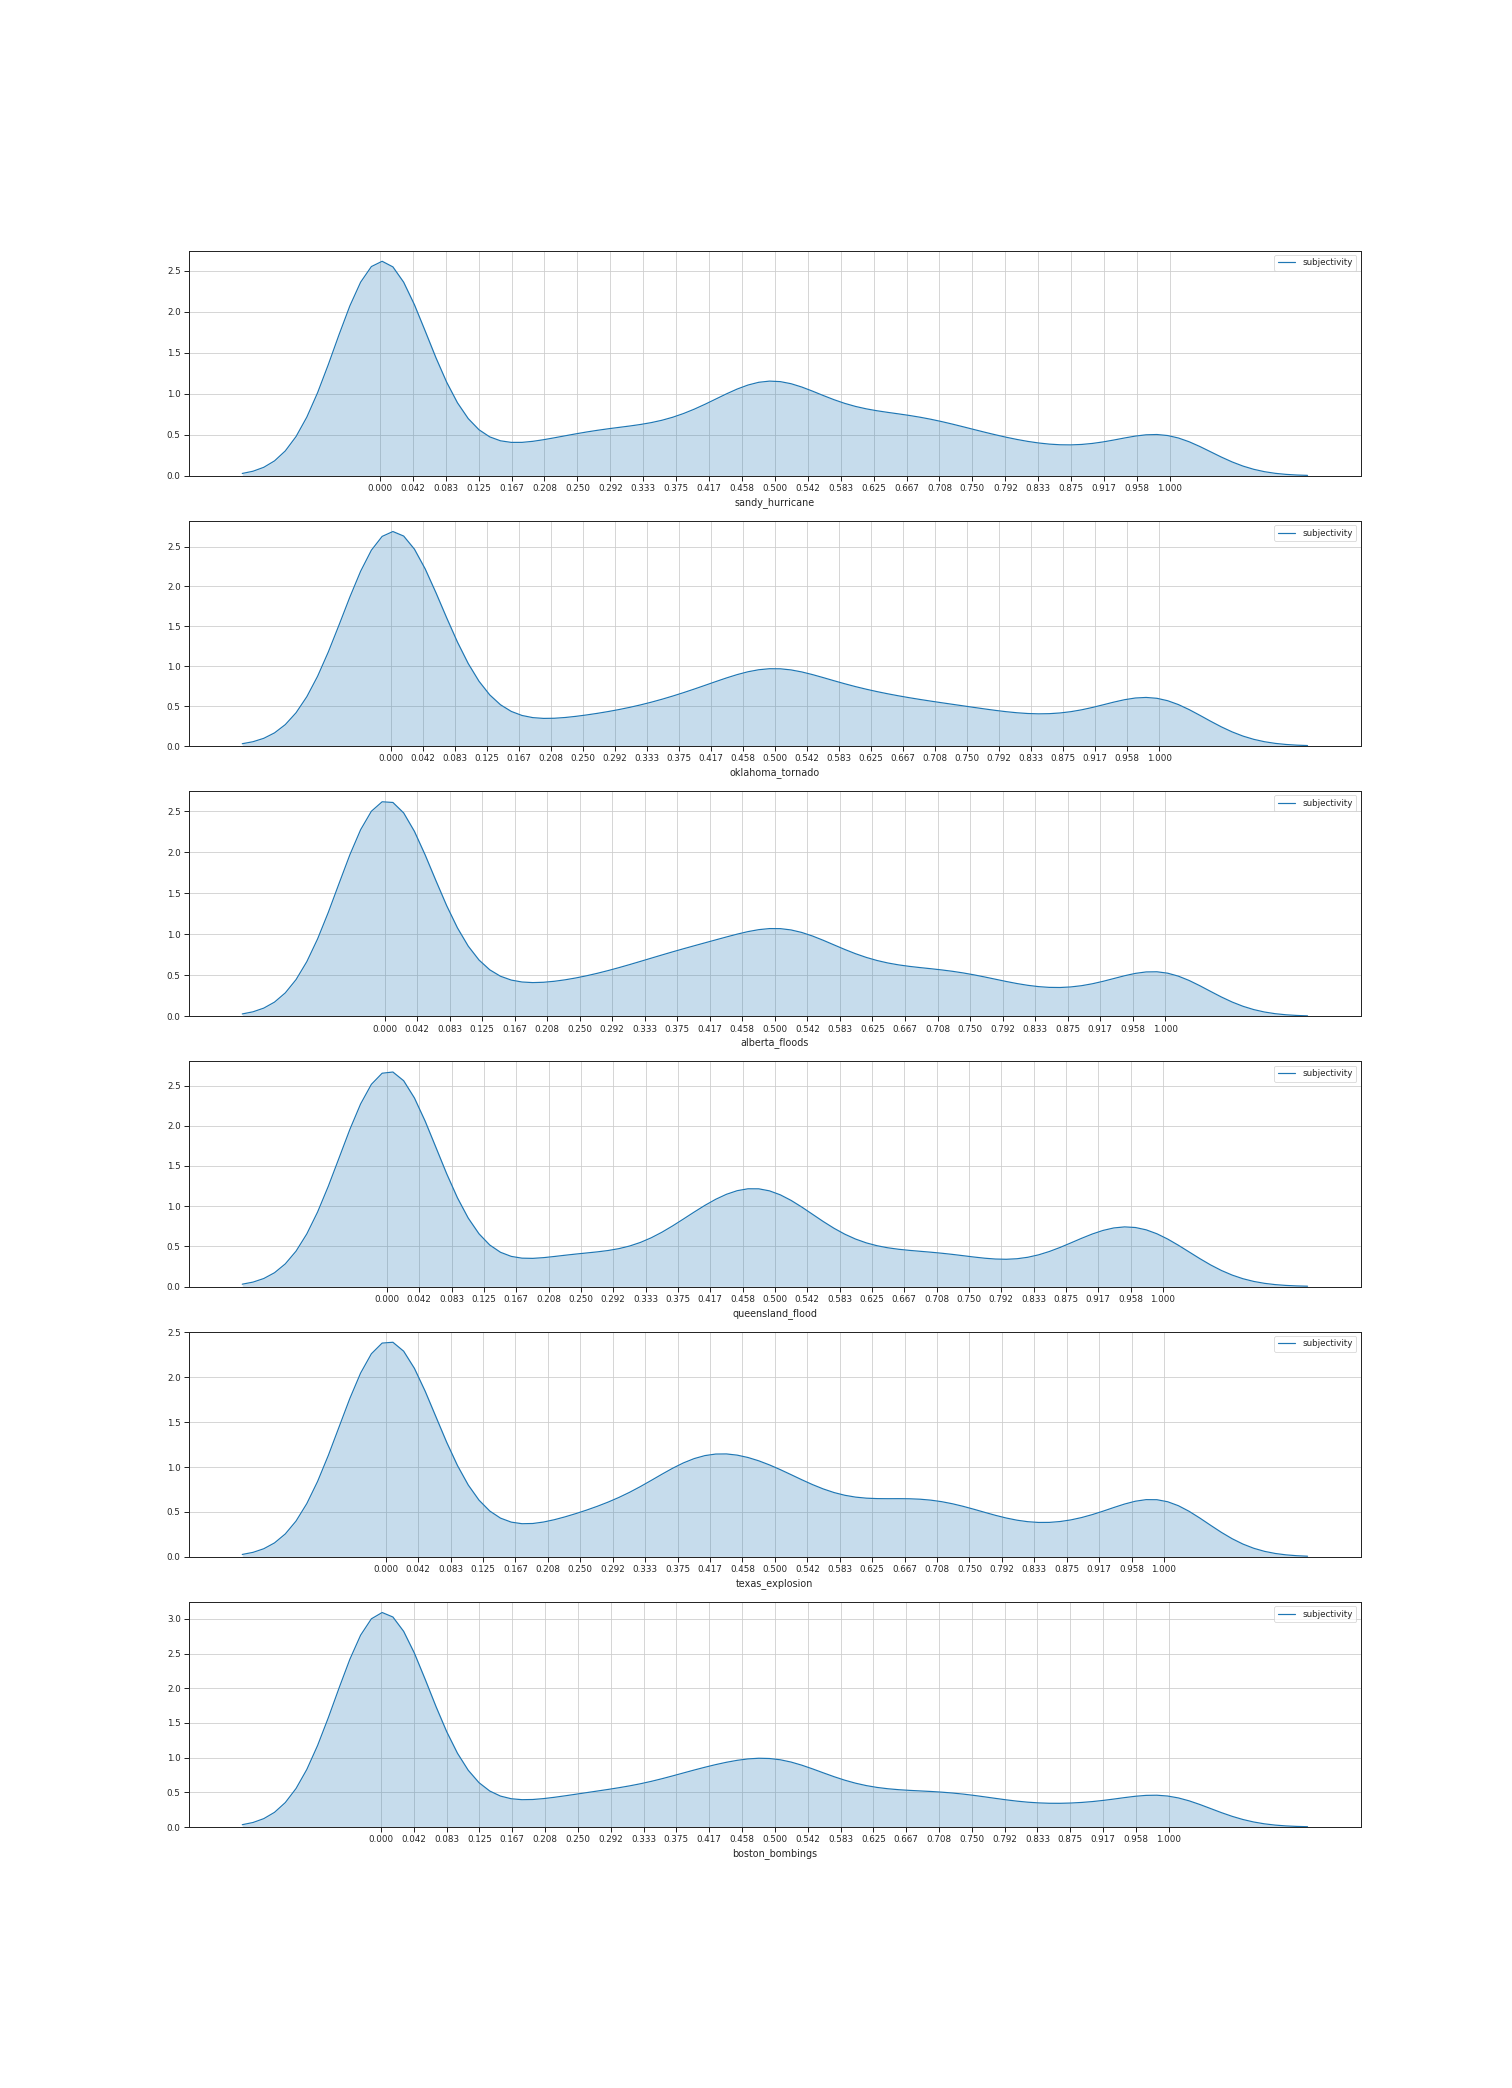
\includegraphics[width=\textwidth]{subjectivity.png}
\caption{Показатель субъективности}\label{subjectivity}
\end{figure}

\begin{figure}
\centering
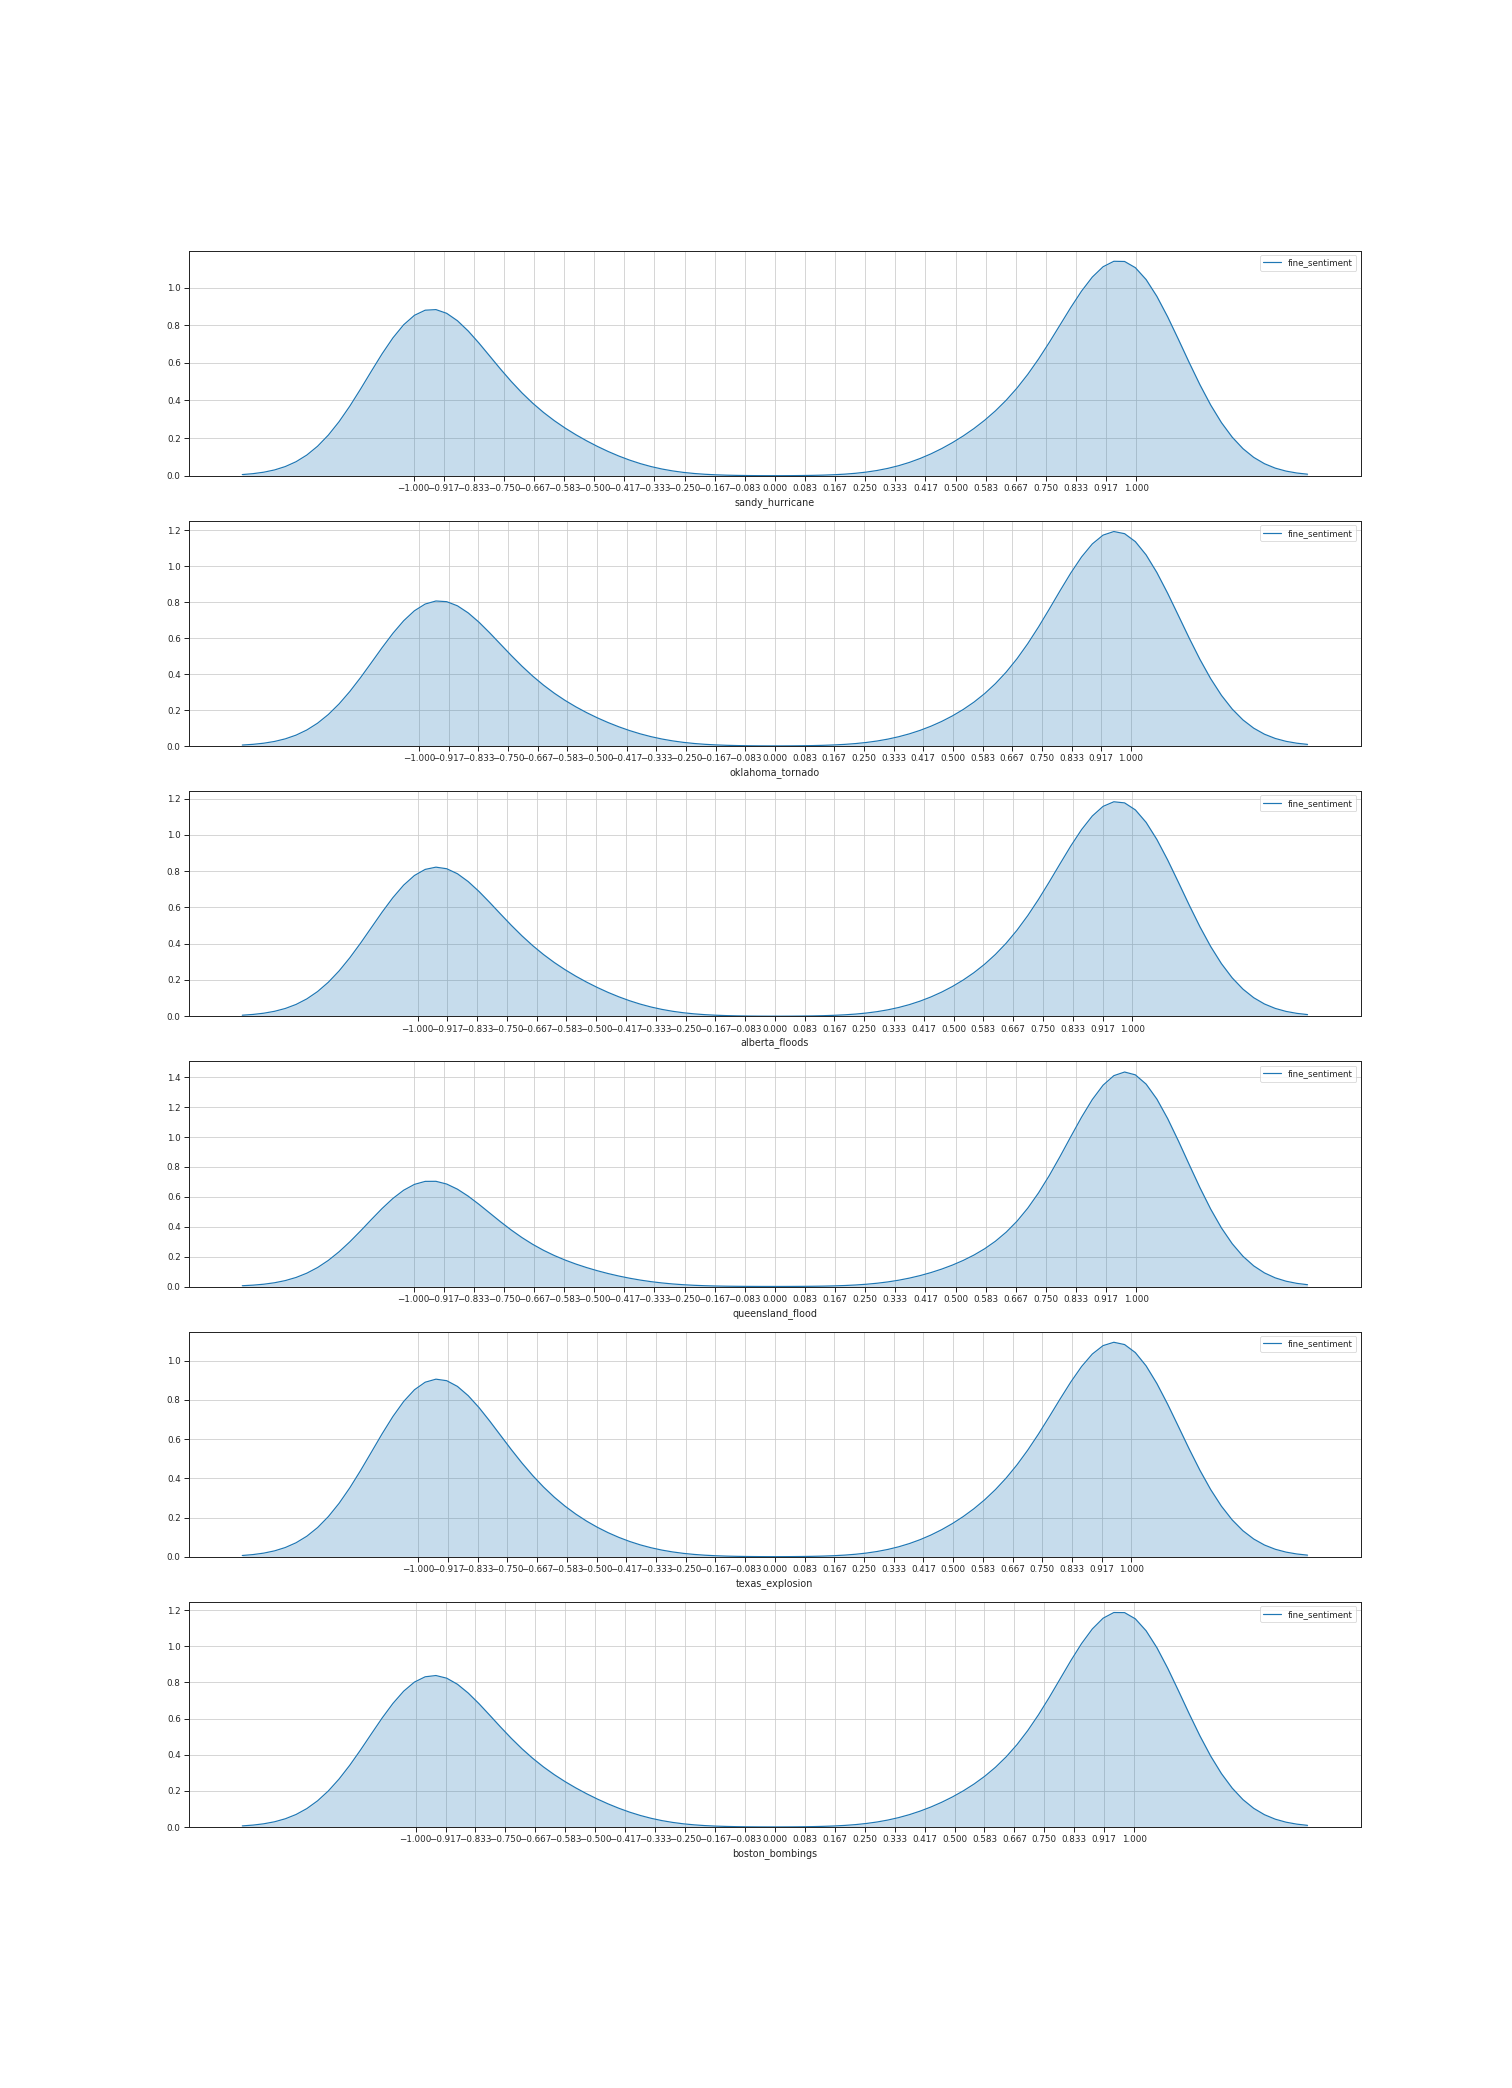
\includegraphics[width=\textwidth]{fine_sentiment.png}
\caption{Показатель `fine\_sentiment` - комбинация sentiment\_score и бинарного показателя sentiment\_value}\label{fine_sentiment}
\end{figure}

\end{document}